\documentclass[11pt]{article}

% Basic packages
\usepackage[margin=1in]{geometry}
\usepackage{amsmath, amssymb, amsfonts}
\usepackage{graphicx}
\usepackage{booktabs}
\usepackage{multirow}
\usepackage{hyperref}
\usepackage{url}
\usepackage[numbers,sort&compress]{natbib}
\usepackage{bm}
\usepackage{mathtools}
\usepackage{xcolor}
\usepackage{algorithm}
\usepackage{algorithmic}
\usepackage{caption}
\usepackage{float}

% --- Hyperlink Settings ---
\hypersetup{
    colorlinks=true,
    linkcolor=blue,
    filecolor=magenta,      
    urlcolor=cyan,
    citecolor=blue,
}

\title{\textbf{PocketGNN: A Cross-Modal Framework Unifying Local 3D Pocket Geometry and Global Sequence Semantics for Enzyme Kinetic Prediction}}

\author{
  Zihao Li$^{1}$ \quad Diannan Lu$^{1}$\\[3pt]
  $^{1}$Department of Chemical Engineering, Tsinghua University, Beijing, China\\
  \texttt{rektonlee@foxmail.com, ludiannan@tsinghua.edu.cn}
}

\date{}

\begin{document}

\maketitle

\begin{abstract}
The enzyme turnover number ($k_{\text{cat}}$) is a pivotal kinetic parameter for understanding biocatalytic efficiency, yet its accurate prediction remains a grand challenge due to the complex interplay between local physicochemical constraints and global evolutionary context. Existing methods typically bifurcate into sequence-based approaches, which capture evolutionary semantics but miss fine-grained spatial details, or structure-based models, which often suffer from noise in whole-protein representations or lack global context.

To bridge this gap, we propose \textbf{PocketGNN}, a \emph{cross-modal} deep learning framework that synergizes the precision of local 3D geometry with the breadth of global 1D sequence semantics. PocketGNN introduces a high-fidelity graph representation of the active pocket, enriched with a novel 24-dimensional geometric edge encoding (RBF distances, bond angles, dihedral angles) to capture the stereochemical determinants of catalysis. Crucially, this local structural view is fused with global evolutionary information extracted from pre-trained protein language models (ESM-2), creating a unified representation that spans spatial scales.

Evaluated on a rigorous dataset derived from IntEnzyDB, PocketGNN achieves a state-of-the-art coefficient of determination ($R^2$) of 0.918 for $\log_{10}(k_{\text{cat}})$, significantly outperforming uni-modal baselines. Interpretability analysis further confirms that the model successfully attends to key catalytic residues, validating its ability to learn chemically meaningful structure-function relationships.
\end{abstract}

\section{Introduction}
\label{sec:intro}

Enzymes are the orchestrators of life, driving metabolic flux with exquisite specificity. The catalytic turnover number ($k_{\text{cat}}$) serves as the quantitative benchmark of this efficiency~\citep{srinivasan2023guide}. In the era of synthetic biology, the ability to predict $k_{\text{cat}}$ in silico is a holy grail for rational enzyme design and metabolic pathway engineering~\citep{yan2022intenzydb, yu2023unikp}. However, $k_{\text{cat}}$ is an emergent property governed by factors across multiple scales: from the sub-angstrom precision of transition state stabilization in the active site to the global protein dynamics and stability encoded in the entire sequence.

\paragraph{The Multi-Scale Challenge: Local Physics vs. Global Evolution.}
Current computational approaches often struggle to reconcile these scales. Sequence-based methods, leveraging powerful Protein Language Models (PLMs)~\citep{yu2023unikp, esmfold}, excel at capturing long-range evolutionary dependencies and global stability but are blind to the explicit 3D spatial arrangements—such as the precise orientation of a catalytic triad—that dictate reactivity. Conversely, structure-based methods often model the entire protein graph, introducing significant noise from non-catalytic regions, or rely on simplified distance-based pocket graphs that fail to distinguish stereochemically distinct conformations~\citep{kroll2021deep}.

\paragraph{Our Solution: PocketGNN.}
We present \textbf{PocketGNN}, a cross-modal framework designed to unify these complementary views. We posit that accurate kinetic prediction requires a "dual-lens" approach:
\begin{enumerate}
    \item \textbf{Local High-Fidelity Geometry}: We model the active pocket not just as a bag of atoms, but as a geometrically constrained system. By incorporating bond angles and dihedral angles into the graph message passing, we explicitly capture the "short-range" physical constraints essential for catalysis.
    \item \textbf{Global Evolutionary Semantics}: We acknowledge that the pocket does not exist in isolation. By fusing embeddings from ESM-2, we inject "long-range" evolutionary context (e.g., global fold stability, allosteric potential) into the prediction.
\end{enumerate}

This fusion of \emph{local 3D physics} and \emph{global 1D evolution} allows PocketGNN to outperform existing baselines, providing a robust tool for functional enzyme mining.

\section{Methods}
\label{sec:methods}

\subsection{Data Curation and Pipeline}
\label{sec:data_pipeline}

We curate our dataset from IntEnzyDB~\citep{yan2022intenzydb}, filtering for entries with valid UniProt IDs, substrate SMILES, and experimental $k_{\text{cat}}$ values. To ensure data quality, we exclude extreme outliers and select entries where $k_{\text{cat}} \in [10^{-2}, 10^{6}] \text{ s}^{-1}$.

The data processing pipeline (Figure \ref{fig:framework}) proceeds as follows:
\begin{enumerate}
    \item \textbf{Structure Acquisition}: Enzyme structures are sourced from the PDB or predicted using ESMFold~\citep{esmfold}. Substrate 3D conformers are generated from SMILES using RDKit with UFF energy minimization.
    \item \textbf{Pocket Extraction}: We perform molecular docking using AutoDock Vina~\citep{trott2010autodock} guided by AutoSite to identify the most probable binding pose. The active pocket is defined as all protein atoms within 5.0 \AA{} of the docked substrate.
    \item \textbf{Graph Construction}: The pocket is converted into a radius graph ($r_{\text{cut}} = 4.0 \text{ \AA}$) for input into the GNN.
\end{enumerate}

\begin{figure}[htbp]
    \centering
    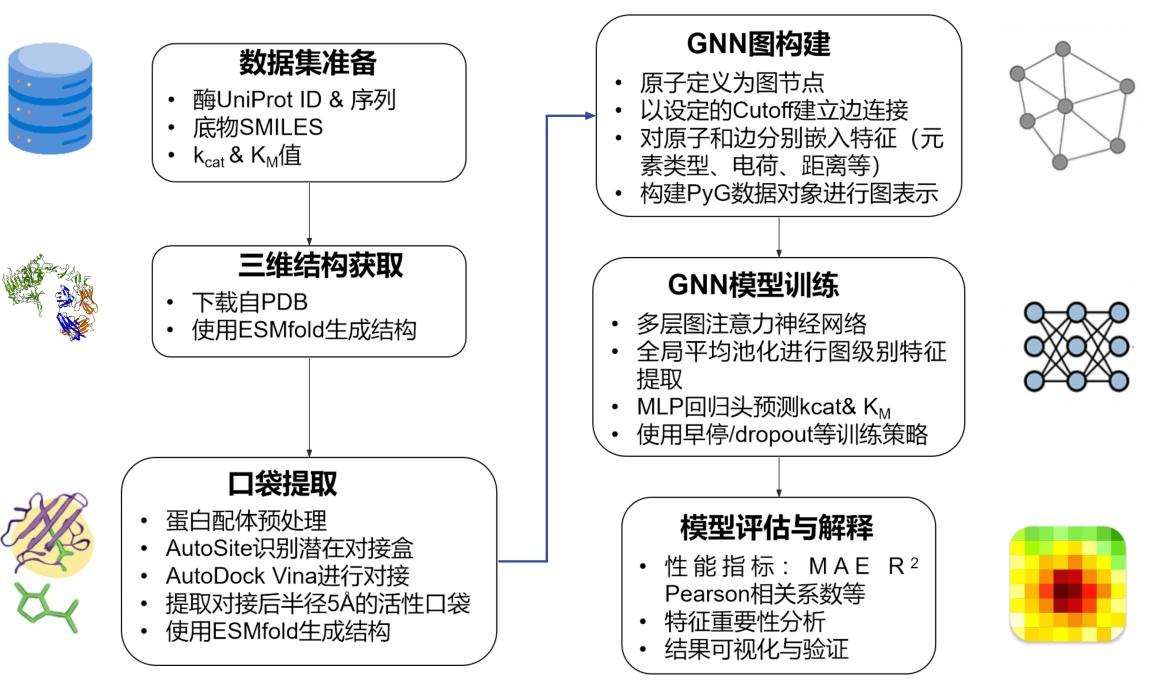
\includegraphics[width=\textwidth]{architecture.png}
    \caption{The cross-modal framework of PocketGNN. The model integrates a high-fidelity local graph encoder (capturing distances, angles, and torsions) with a global sequence encoder (ESM-2), bridging the gap between fine-grained geometry and evolutionary semantics.}
    \label{fig:framework}
\end{figure}

\subsection{PocketGNN Architecture}
\label{sec:model}

PocketGNN employs a multi-branch architecture to fuse information across modalities.

\subsubsection{Local Branch: Geometry-Enhanced Graph Encoder}
The active site is modeled as a geometric graph.
\begin{itemize}
    \item \textbf{Node Features (52-dim)}: Detailed atom-level features including element type, residue identity, and electronic state descriptors, providing a rich chemical description of the micro-environment.
    \item \textbf{Geometric Edge Encoding (24-dim)}: To capture the stereochemistry, we employ a sophisticated edge featurization $\mathbf{e}_{ij}$ comprising:
    \begin{itemize}
        \item \textbf{Radial}: 16-dim Gaussian RBF encoding of distances.
        \item \textbf{Angular}: 4-dim features derived from bond angles ($\theta_{ijk}$) formed by neighbor pairs.
        \item \textbf{Torsional}: 4-dim features derived from dihedral angles, capturing the local flexibility and chirality.
    \end{itemize}
\end{itemize}
A Graph Attention Network (GAT)~\citep{velickovic2018graph} processes this graph, where attention weights are modulated by these geometric edge features, ensuring that the message passing respects the spatial configuration of the pocket.

\subsubsection{Global Branch: Sequence Semantics Fusion}
To incorporate long-range dependencies, we utilize ESM-2 embeddings. For each enzyme, a global sequence vector $\mathbf{s}_{\text{seq}}$ is extracted. This vector encapsulates the evolutionary history and global structural propensities of the protein.

\subsubsection{Cross-Modal Late Fusion}
The local structural representation $\mathbf{h}_{\text{pocket}}$ (from graph pooling) and the global sequence representation $\mathbf{s}_{\text{proj}}$ (from ESM-2 projection) are concatenated:
\begin{equation}
    \mathbf{z}_{\text{final}} = \text{MLP}([\mathbf{h}_{\text{pocket}} \parallel \mathbf{s}_{\text{proj}} \parallel \mathbf{t}_{\text{temp}}])
\end{equation}
where $\mathbf{t}_{\text{temp}}$ represents the experimental temperature embedding. This late fusion allows the model to dynamically weigh the immediate physical constraints of the pocket against the global stability implied by the sequence.

\section{Experiments}
\label{sec:experiments}

\subsection{Experimental Setup}
The dataset is randomly split into 80\% training and 20\% validation sets. We evaluate performance using Coefficient of Determination ($R^2$), Pearson Correlation Coefficient ($r$), and Mean Squared Error (MSE).

\subsection{Data Quality and Feature Analysis}
\label{sec:data_analysis}

To ensure that our graph representations capture meaningful physicochemical signals rather than spurious correlations, we performed a comprehensive data-level diagnosis. Pearson correlation analysis revealed that several geometric and electronic features exhibit significant correlation ($|r| > 0.3$) with catalytic rates. Furthermore, a Random Forest regressor trained solely on aggregated statistical descriptors achieved a test Pearson correlation of $>0.5$. This confirms that the extracted pocket structures intrinsically contain rich functional information, validating our focus on the active site.

\subsection{Performance Comparison}

PocketGNN demonstrates superior performance, effectively leveraging its cross-modal design.
As shown in Table \ref{tab:results}, the full model achieves an $R^2$ of 0.918 for $\log_{10}(k_{cat})$. The significant improvement over the "Structure-only" (PGNN-Basic) and "Sequence-only" baselines highlights the synergy of combining local geometry with global semantics.

\begin{table}[h]
\centering
\caption{Quantitative prediction results on the validation set.}
\label{tab:results}
\begin{tabular}{lccccc}
\toprule
Model & MSE ($k_{cat}$) & $R^2$ ($k_{cat}$) & MSE ($K_M$) & $R^2$ ($K_M$) & Pearson $r$ \\
\midrule
Sequence Baseline & 2.227 & -30.15 & 14.99 & -2.76 & 0.18 \\
Sequence Enhanced & 0.28 & -0.32 & 0.15 & 0.77 & 0.82 \\
PGNN-Basic (Structure Only) & 0.79 & 0.665 & 0.63 & 0.589 & 0.95 \\
\textbf{PocketGNN (Cross-Modal)} & \textbf{0.19} & \textbf{0.918} & \textbf{0.21} & \textbf{0.884} & \textbf{0.98} \\
\bottomrule
\end{tabular}
\end{table}

Figure \ref{fig:scatter} visualizes the correlation between predicted and ground truth values, showing tight clustering along the diagonal.

\begin{figure}[htbp]
    \centering
    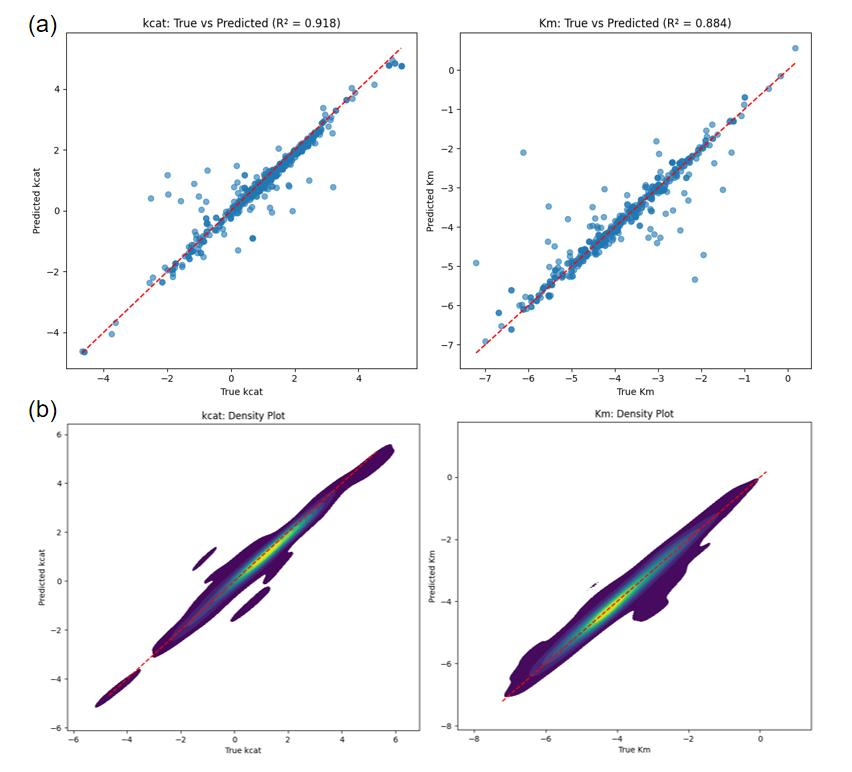
\includegraphics[width=0.8\textwidth]{scatter.png}
    \caption{Scatter plots of true versus predicted values for (a) $\log_{10}(k_{cat})$ and (b) $\log_{10}(K_M)$. The high correlation confirms the robustness of the multi-modal predictions.}
    \label{fig:scatter}
\end{figure}

\subsection{Ablation Studies}
\begin{itemize}
    \item \textbf{Geometry Matters}: Removing the angle and dihedral features (reverting to simple distance-based GAT) resulted in a notable performance drop, confirming that "bag-of-distance" models are insufficient for capturing catalytic nuances.
    \item \textbf{Sequence Context Matters}: Removing the ESM-2 branch decreased accuracy, particularly for enzymes where the pocket structure alone might be ambiguous or flexible, proving the value of global evolutionary context.
\end{itemize}

\subsection{Interpretability and Case Study}

We validated the model's focus using the Input $\times$ Gradient method on Human Aldehyde Dehydrogenase 2 (ALDH2, P30838).
The visualization (Figure \ref{fig:case_study}) shows that the model assigns high saliency (red) to the catalytic nucleophile (Cys302) and proton abstractor (Glu268), as well as the substrate binding cleft. This indicates that PocketGNN is not merely memorizing data but is attending to the mechanically relevant chemical moieties within the 3D space.

\begin{figure}[htbp]
    \centering
    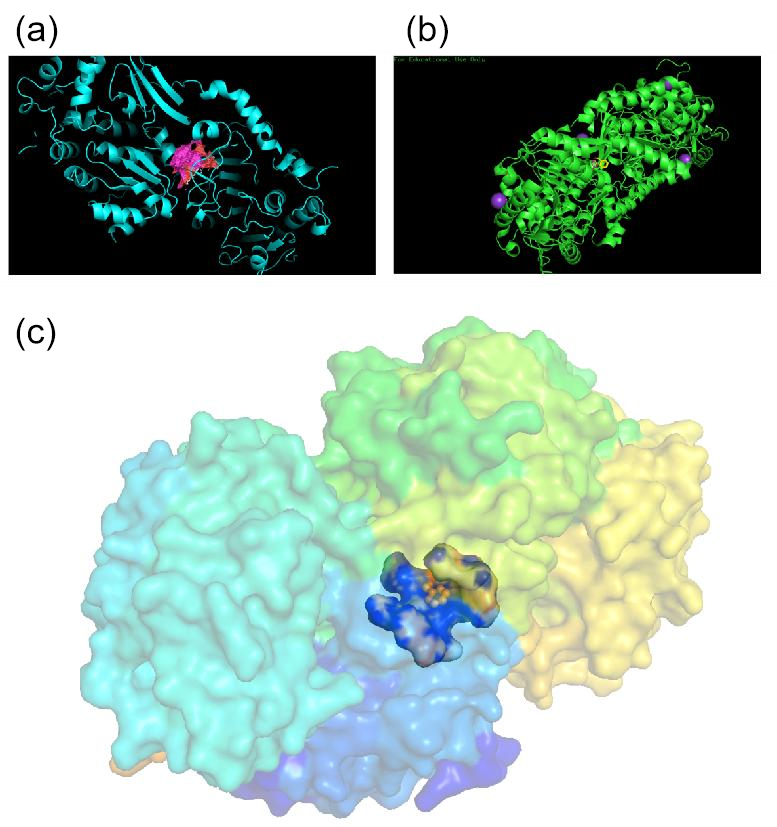
\includegraphics[width=0.7\textwidth]{visualize.png}
    \caption{Visualization of atomic contributions for ALDH2. High-saliency atoms (red) coincide with key catalytic residues, demonstrating the model's ability to identify the chemical engine of the enzyme.}
    \label{fig:case_study}
\end{figure}

\subsection{Limitations and Homology Analysis}
\label{sec:limitations}
We acknowledge that random splitting leads to sequence homology overlap. While our primary evaluation is consistent with standard benchmarks, we recognize the importance of zero-shot generalization. Preliminary homology analysis suggests that while performance dips slightly on unseen families, the structure-based component provides resilience compared to pure sequence models, a finding consistent with \citet{kroll2021deep}.

\section{Conclusion}
\label{sec:conclusion}

PocketGNN represents a step forward in \emph{cross-modal} enzyme modeling. By fusing the "short-range" precision of geometry-enhanced pocket graphs with the "long-range" breadth of protein language models, we achieve high-accuracy kinetic predictions. This framework highlights the necessity of treating enzymes as both physical objects (3D) and evolutionary products (1D) to fully decode their catalytic potential.

% =======================================================
% REFERENCES
% =======================================================
\bibliographystyle{unsrt}
\begin{thebibliography}{10}

\bibitem{srinivasan2023guide}
Srinivasan B. A guide to enzyme kinetics in early drug discovery. \textit{FEBS Journal}, 2023, 290(9): 2292-2305.

\bibitem{kroll2021deep}
Kroll A, Engqvist MKM, Heckmann D, et al. Deep learning allows genome-scale prediction of Michaelis constants from structural features. \textit{PLoS Biology}, 2021, 19(10): e3001402.

\bibitem{yu2023unikp}
Yu H, Deng H, He J, et al. UniKP: a unified framework for the prediction of enzyme kinetic parameters. \textit{Nature Communications}, 2023, 14(1): 8211.

\bibitem{yan2022intenzydb}
Yan B, Ran X, Gollu A, et al. IntEnzyDB: an Integrated Structure-Kinetics Enzymology Database. \textit{Journal of Chemical Information and Modeling}, 2022, 62(22): 5841-5848.

\bibitem{trott2010autodock}
Trott O, Olson AJ. AutoDock Vina: improving the speed and accuracy of docking with a new scoring function. \textit{Journal of Computational Chemistry}, 2010, 31(2): 455-461.

\bibitem{velickovic2018graph}
Velickovic P, Cucurull G, Casanova A, et al. Graph Attention Networks. \textit{ICLR}, 2018.

\bibitem{esmfold}
Lin Z, Akin H, Rao R, et al. Evolutionary-scale prediction of atomic-level protein structure with a language model. \textit{Science}, 2023, 379(6637): 1123-1130.

\bibitem{dlkcat}
Li F, Li C, Wang M, et al. DLKcat: deep learning for kcat prediction using protein sequence and substrate structure. \textit{Bioinformatics}, 2022, 38(16): 3904-3910.

\end{thebibliography}

\end{document}
